\section{System's scheme}
\label{sec:sectionb}

The experimental procedure of visual stimuli display involved four main components in communication of parameters, configurations and triggered synchronization: A governing machine and a stimulus display matlab instances, a Bpod device and the set of two-photon laser microscopy appliances and software. 

\begin{figure}[H]
	\centering
		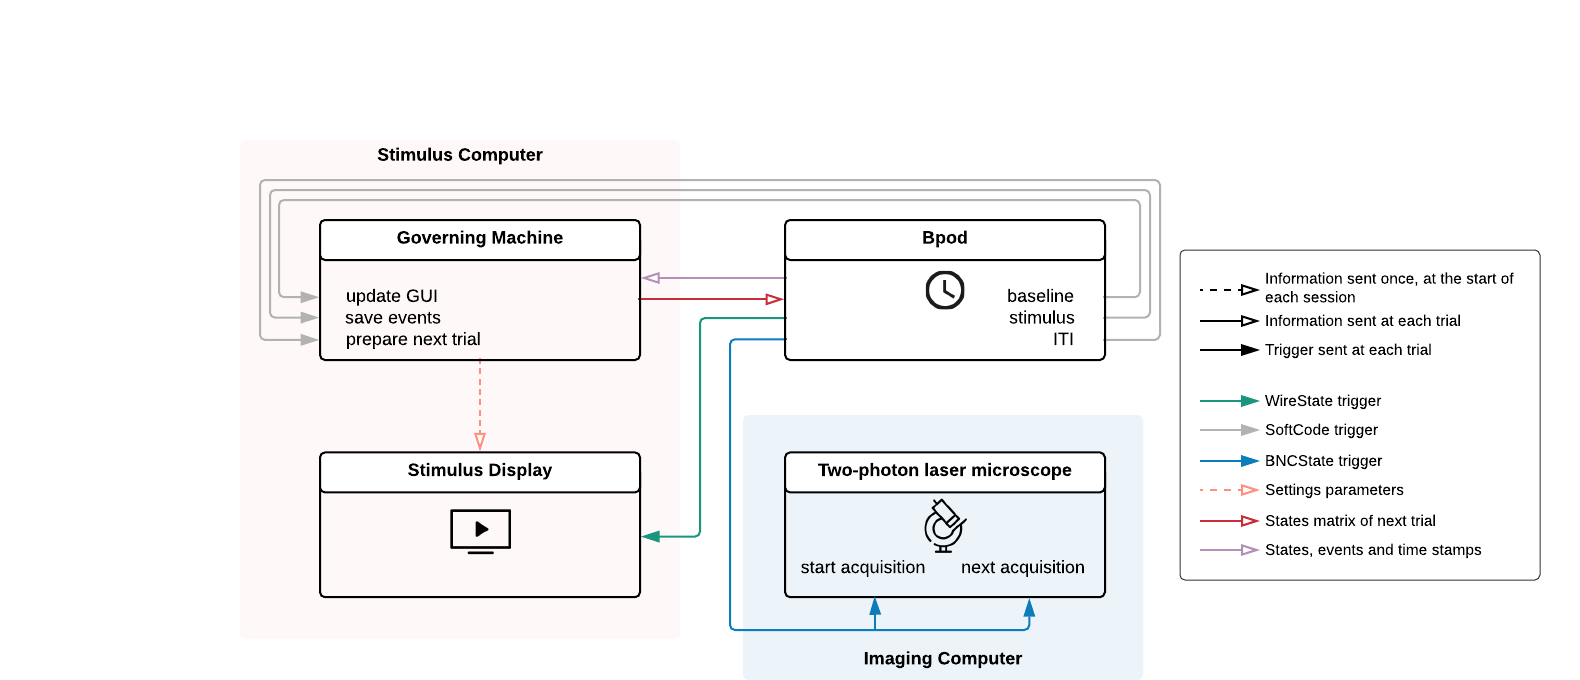
\includegraphics[width=1\linewidth]{3.Chapter/systemtechnical.png}
	\caption[c1]{Setup and connections scheme of devices used for stimuli presentation and real-time imaging.}
	\label{fig:systemtechnical}
\end{figure}

Controlled by one of the computers, called here stimulus computer, were the governing machine and the stimulus display.

The governing machine held the Graphical User Interface (GUI) as well as all of the computations and running protocols with Bpod's software for saving the stimuli settings and preparing the stimuli configurations and states matrices for the different trials. 

The stimulus display was produced in a second monitor connected to this stimulus computer and operated within a second matlab instance of routines coded with Psychtoolbox software for interfacing between Matlab and the computer screen. This Matlab instance loaded, at the beginning of the session, all of the stimuli settings that were saved in the bpod's Matlab instance. With a counter, the script iterated the full trials structure, displaying the applicable stimuli at the proper times. This timing synchronization was enabled by triggers received in a NI-DAQ data acquisition board. 

The bpod apparatus produced these triggers, connected to the system and taking advantage of a precise internal clock. Having received each trial's state-matrix specifications from the governing machine with enough buffer time, bpod produced the appropriately timed states - the main ones being the baseline, the stimulus and the ITI - and sent the required triggers at each stage. At each trial, in the beginning of the baseline period, a trigger was sent to the governing machine to update the GUI to show the current trial stimuli specifications; during the stimulus presentation, another trigger was sent to save the events of the previous trial and during the ITI an instruction was sent for the governing machine to prepare the next trial by computing the next states matrix with the new trial's stimuli configurations. Bpod also sent, at the beginning of the stimulus display state, the trigger for the stimulus computer second matlab instance to display the loaded and prepared stimulus in the screen visualized by the animal. Finally, at the beginning of the baseline and in the end of the ITI of the proper trials, a trigger was sent to the called imaging computer that held the software controlling the two-photon laser microscope for respectively starting and afterwards completing and proceeding to the next brain scanning acquisition. 

The two-photon laser microscope held different components: The laser apparatus with the mirrors, lenses, beam-splitter and remaining light path enforcers; the objective enabling both a bright field and a two-photon configurations; the synchronization device BLACK BOX[?], a NI-DAQ data acquisition board for receiving Bpod's triggers, and finally the imaging computer that operated the controlling software application ScanImage 4 for laser scanning microscopy. This was also the computer that saved the raw image sets acquired from the two-photon scannings at each protocol session.

The sent information and triggers used the different physical wiring possibilities: Firstly, SoftCodes were sent from bpod to the governing machine's computer, via the USB port that connected these devices. From bpod to the stimulus display NI-DAQ board, WireStates were used, and, to the two-photon NI-DAQ board, BNCState triggers were sent. On the other hand, the information about states, events and trial time stamps was sent at each trial via USB from the Bpod device to the bpod's governing machine matlab instance and then saved with its own software. 
From the governing machine, information was sent as the following trial's state matrix, to the bpod device also via USB and the next trial's settings were sent to the stimulus display matlab instance by saving them at the beggining of  each protocol session in a file that was then loaded in the stimulus display matlab before starting the session.